\newpage


%%%%%%%%%%%%%%%%%%%%%%%%%%%%%%%%%%%%%%%%%%%%%%%%%%%%%%%%%%%%%%%%%%%%%%%%%%%%%%%%%%%%%%%
%%%%%%%%%%%%%%%%%%%%%%%%%%%%%%%%%%%%%%%%%%%%%%%%%%%%%%%%%%%%%%%%%%%%%%%%%%%%%%%%%%%%%%%
%%%%%%%%%%%%%%%%%%%%%%%%%%%%%%%%%%%%%%%%%%%%%%%%%%%%%%%%%%%%%%%%%%%%%%%%%%%%%%%%%%%%%%%
\section{Regressão logística-fourier e SE com classificador $f_{\VECTOR{c}}(x):~\mathbb{R} \rightarrow \mathbb{R}$}
\label{sec:theo:reglogr1r1fourier:1}

\index{Regressão!Logística $f_{\VECTOR{c}}(x):~\mathbb{R} \rightarrow \mathbb{R}$}

\begin{theorem}[Classificação de dados em $\mathbb{R}$:]\label{theo:reglogr1r1fourier:1}
~\\
\noindent
\begin{minipage}{0.45\textwidth}
\centering
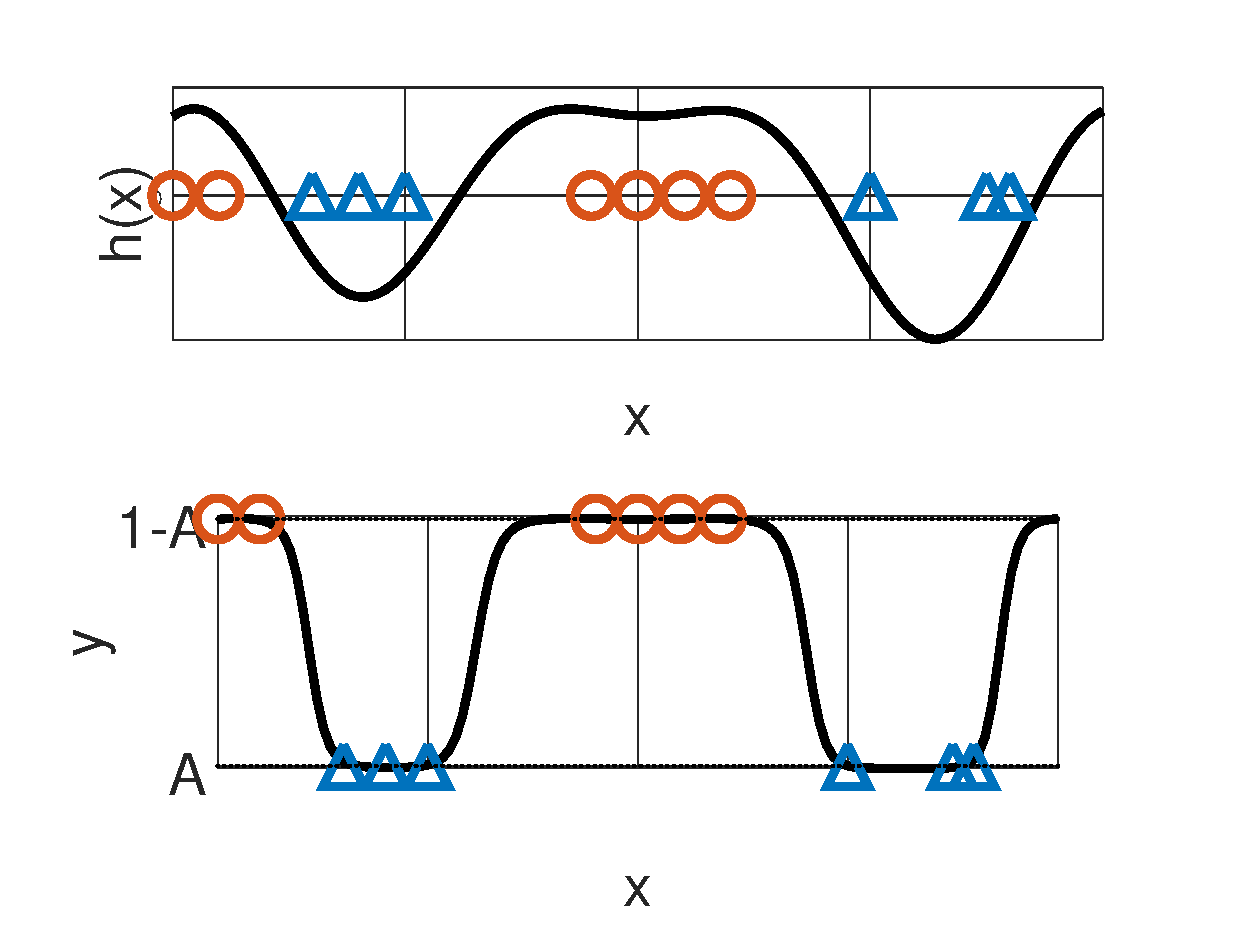
\includegraphics[width=0.95\linewidth]{chapters/classificacao/mfiles/reglogr1r1fourier/reglogr1r1fourier.eps} 
\end{minipage}
\begin{minipage}{0.55\textwidth}
Dados, um conjunto de $L$ dados $x_l \in \mathbb{R}, 1 \leq l \leq L$,
repartidos em dois grupos etiquetados com os símbolos $\bigtriangleup$ e $\bigcirc$, 
e separáveis por um hiperplano.
Se desejamos criar um classificador mediante 
a função  $f_{\VECTOR{c}}:\mathbb{R} \rightarrow \mathbb{R}$,
com domínio $x \in \mathbb{R}$, contradomínio $y \in \mathbb{R}$ e 
parâmetros agrupados no vetor $\VECTOR{c}=[c_1~ c_2~ ...~ c_{2 K+1}]^{\transpose}\in \mathbb{R}^{2 K+1}$,
como definido na Eq. (\ref{eq:reglogr1r1fourier:1}),
\begin{equation}\label{eq:reglogr1r1fourier:1}
y\equiv f_{\VECTOR{c}}(x)= \frac{1}{1+e^{-h_{\VECTOR{c}}(x) }},
\end{equation}
\end{minipage}
\begin{equation}
\quad h_{\VECTOR{c}}(x)=\frac{c_1}{2}+ \sum_{k=1}^{K} \left\{ 
c_{2k} sin\left(k \frac{2 \pi x}{L_x}\right) + 
c_{2k+1} cos\left(k \frac{2 \pi x}{L_x}\right)
\right\},
\end{equation}
ou seu equivalente: $logit(y)=h_{\VECTOR{c}}(x)$, onde\footnote{Tem 
que ser maior para evitar erros de $f_{\VECTOR{c}}(x)$ nos extremos. 
Ex.: $L_x =1.1 || max(x_i)-min(x_i)||$.}
 $L_x > || max(x_i)-min(x_i)||$.

Podemos atribuir a cada valor $x_l$ uma etiqueta $y_l\in \{A,1-A\}$, 
onde $0<A\ll 0.5$ é escolhido por nós,
e afirmar que o vetor $\VECTOR{c}= \VECTOR{\hat{c}}$,
que minimiza o erro quadrático $e(\VECTOR{c})$,
\begin{equation}\label{eq:reglogr1r1fourier:1e}
e(\VECTOR{c}) =  \sum_{l=1}^{L} w_l||h_{\VECTOR{c}}(x_l) -logit(y_l)||^2,
\end{equation}
ponderado usando os pesos $w_l \in \mathbb{R}_+$, 
pode ser achado\footnote{A demostração pode ser vista na Prova \ref{proof:theo:reglogr1r1fourier}.}  
com
\begin{equation}\label{eq:reglogr1r1fourier:2}
\VECTOR{\hat{c}} =  \left[ \MATRIX{A}^{\transpose} \MATRIX{W}\MATRIX{A}\right]^{-1} \MATRIX{A}^{\transpose} \MATRIX{W}\VECTOR{z},
\quad
\MATRIX{A}=
\begin{bmatrix}
\VECTOR{a}_{K}(x_1) \\
\VECTOR{a}_{K}(x_2) \\
\vdots \\
\VECTOR{a}_{K}(x_l) \\
\vdots \\
\VECTOR{a}_{K}(x_L) \\
\end{bmatrix},
\quad
\MATRIX{W}=\funcdiag \left(
\begin{bmatrix}
w_1  \\
w_2  \\
\vdots  \\
w_l  \\
\vdots \\
w_L \\
\end{bmatrix}
\right),
\quad
\VECTOR{z}=
\begin{bmatrix}
logit(y_1)  \\
logit(y_2)  \\
\vdots  \\
logit(y_l)  \\
\vdots \\
logit(y_L) \\
\end{bmatrix},
\end{equation}
\begin{equation}
\VECTOR{a}_{K}(x)=
\begin{bmatrix}
\frac{1}{2} & 
sin\left( \frac{2 \pi x}{L_x}\right) & 
cos\left( \frac{2 \pi x}{L_x}\right) &
%sin\left(2 \frac{2 \pi x}{L_x}\right) & 
%cos\left(2 \frac{2 \pi x}{L_x}\right) &
\dots &
sin\left(K \frac{2 \pi x}{L_x}\right) & 
cos\left(K \frac{2 \pi x}{L_x}\right)
\end{bmatrix}.
\end{equation}
\end{theorem}
\begin{tcbattention}
\begin{itemize}
\item Dado que a função de classificação $f_{\VECTOR{c}}(x)$ vai entre $0$ e $1$,
podemos reinterpretar este valor como se fosse uma probabilidade;
neste caso, $f_{\VECTOR{c}}(x_l)$ representa, $P(y_l=\bigcirc|x_l)$, 
a probabilidade de que $y_l=\bigcirc$ dado que tivemos como entrada o valor $x_l$.
%\item O limiar da classificação de $f_{\VECTOR{c}}(x)$ 
%está no hiperplano $h_{\VECTOR{c}}(x)=0$,
%provocando neste ponto um $f_{\VECTOR{c}}(x)=0.5$.
\item $L_x$ indica o periodo de repetição do classificador,
por este motivo o classificador é interessante quando o domínio dos dados ($x_l$) está restrito.
\end{itemize}
\end{tcbattention}

